\documentclass[../main.tex]{subfiles}

\graphicspath{../images}

\begin{document}

\chapter{初步认识计算机}

在真正学习计算机的有关内容之前,我们需要对计算机有一个最初步的认识。计算机是一个复杂的系统,它由许多不同的部件和组件组成,这些部件和组件共同工作以完成各种任务。

\section{计算机的鼻祖}

人们一直在思考怎样进行更高效的计算。在古代,算盘、算筹等工具被用来进行计算。后来,随着科学技术的发展,人们对计算的需求越来越高,开始设计和制造更复杂的计算设备。查尔斯·巴贝奇(Charles Babbage)被认为是计算机的鼻祖,他在19世纪设计了第一台机械计算机——差分机和分析机。虽然他的设计在当时没有被完全实现,但他的思想为后来的计算机发展奠定了重要的基础。

我们一般认为,图灵是赋予现代计算机灵魂的人。他在1936年提出了“图灵机”的概念,图灵机是一个抽象的计算模型,能够模拟任何计算机的计算过程。自此,问题被分为两类:能用图灵机解决的(或者称作“图灵可计算的”)和不能用图灵机解决的;遇到前者,我们就可以掏出图灵机计算。图灵机的提出为现代计算机科学奠定了基础。关于图灵机本身的内容已经超出了本节课的范围,我们在这里不做过多介绍。

然而,图灵机更多的是一种抽象概念,真正把计算机变成现实的是冯·诺依曼。冯·诺依曼在1945年总结前人经验,提出并推广了“普林斯顿架构”。后来这个架构也被称作“冯·诺依曼架构”,也就是我们现在所说的计算机的基本结构。冯·诺依曼架构的核心思想是将程序和数据存储在同一块内存中,这样计算机就可以根据程序的指令来操作数据。冯·诺依曼架构是现代计算机的基础,目前几乎所有的计算机都遵循这一架构。

\section{现代计算机的组成}

计算机的组成可以分为\textbf{硬件}和\textbf{软件}两大部分。硬件是指计算机的物理部件,如中央处理器(CPU)、内存、硬盘、显示器等;软件是指计算机上运行的程序和操作系统,如Windows、Linux、macOS等操作系统,以及Chrome、VS Code、Tencent QQ等应用程序。

\subsection{计算机的硬件}

计算机的\textbf{硬件},也可以叫做\textbf{设备},可以简单分为两类:一类叫做\textbf{主机设备},是计算机用来进行计算等工作的设备;另一类叫做\textbf{外设设备}(也可以叫做\textbf{输入输出设备}),是计算机与外界进行信息交互的设备。通常说来,前者是藏在机箱里看不见的,后者是我们能够直接看见的。

一个计算机的主机设备如图所示:
\begin{figure}[htbp]
    \centering
    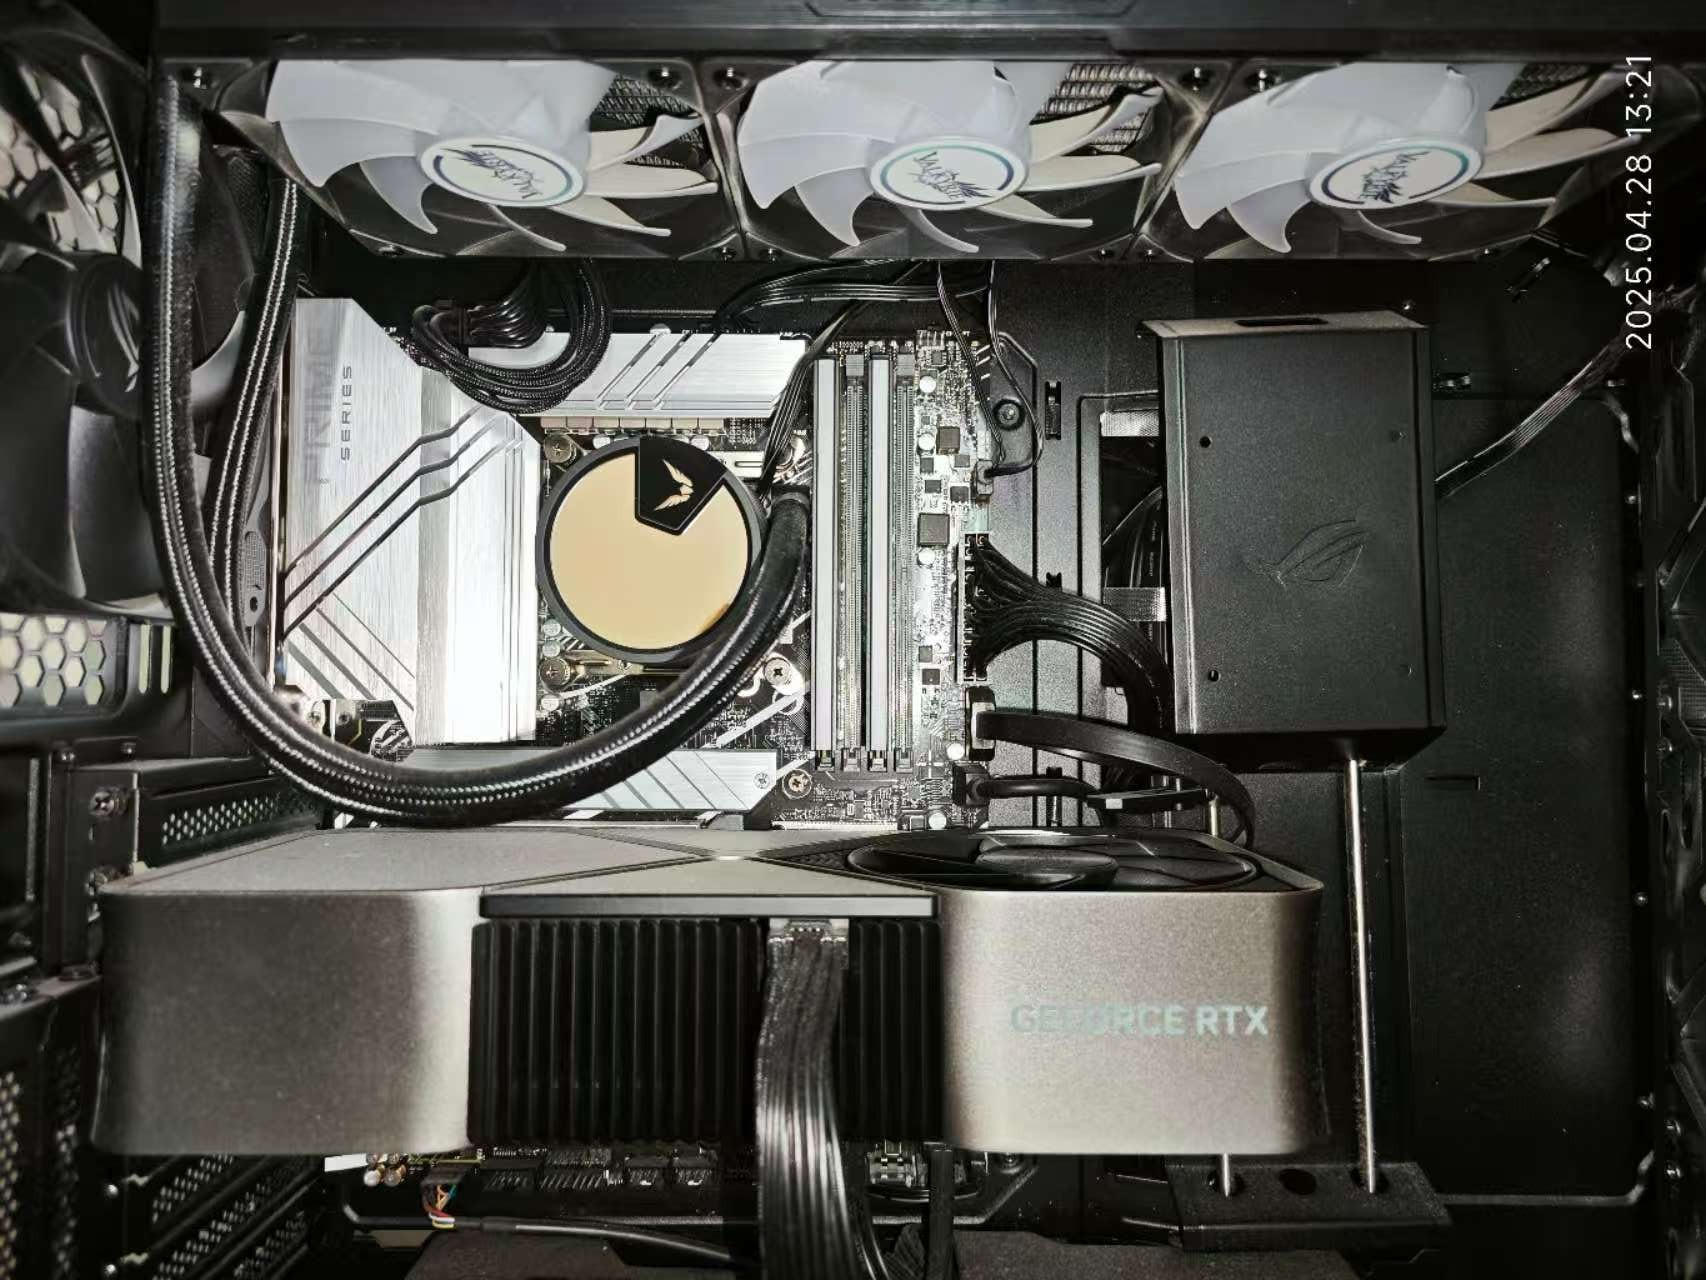
\includegraphics[width=0.8\textwidth]{images/hardware1.jpg}
    \caption{计算机的主机设备}
    \label{fig:computer-hardware}
\end{figure}

下面将会逐个介绍这些设备。

\subsubsection{中央处理器(CPU)}

CPU是计算机的最核心部件,它从存储设备读取指令和数据,并且执行这些指令。尽管现代处理器对代码和数据会有不同的处理,但是从程序员视角来看,其本质上都以二进制存储。代码由一条一条的指令组成,CPU 按照顺序一条一条执行从存储设备中读取的指令(至少从软件和程序员等使用者的视角看是这样),指令可以是修改 CPU 的状态,进行运算,或者是从其他硬件读取信息或者输出信息。如果希望进一步学习CPU如何运作等相关知识,可以参考著名的教材《CSAPP》,也可以修习《计算机系统导论》(ICS)这门课。

\subsubsection{内存(RAM)}

内存是计算机的临时存储器,它用于存储正在运行的程序和数据。它能够被CPU直接访问,因此速度较快。对于程序员而言,内存可以被抽象为一堆连续的存储单元,每个存储单元都有一个唯一的地址;执行程序时,程序的一部分或者全部被放进内存中,CPU就在内存中找寻需要的数据或者指令,如同在排列整齐的暑假上寻找需要的书籍。

现代计算机内存读写速度很快,但是已经跟不上CPU的速度,因此又引入了高速缓存来加速内存的读写速度。高速缓存是内存和CPU之间的一个小型存储器,它存储了最近使用的数据和指令,以便CPU可以更快地访问它们。在断电以后,内存中存储的数据会丢失,因此内存也被称为是易失性的存储器。

特别注意:上述文本中的“内存”指的是“随机存取存储器”(RAM)。这里的“随机”指的是“随机存取”,也就是可以在任意时刻访问任意地址的存储器,而不是“顺序存取”的存储器(例如磁带)。同时,“内存”这个词在部分语境下又不同的含义,例如在BIOS语境下的“内存”指的是“只读存储器”(ROM),在移动设备(手机)等语境下的“内存”指的是“闪存”,这实际上是外存。

\subsubsection{外存}

外存是现代计算机的主要存储设备,用于存储操作系统、应用程序和数据等内容。其读写速度往往比内存慢得多,但是它的存储容量更大且往往是非易失的(相对内存而言)。

现代计算机的主要外存设备是硬盘。硬盘可以分为机械硬盘(HDD)和固态硬盘(SSD)。机械硬盘使用磁头在旋转的磁盘上读取和写入数据,而固态硬盘使用闪存芯片来存储数据。固态硬盘的读写速度比机械硬盘快得多,现在价格也便宜得多,但是使用寿命较短,且因为电荷流失等问题无法接受长期不通电等情况,不适宜作为长期存档介质(个人使用寿命和HDD无明显差异,基本都能用到彻底换机),除非花高价买高端的企业级SSD,但仍需定期通电。

除硬盘外,还有其他外部存储设备。例如:
\begin{itemize}
    \item U盘:一种小型的闪存存储设备,通常通过USB接口连接到计算机上。虽然和SSD都使用闪存颗粒,但是SSD通过主控优化、多通道技术等实现更高的性能,U盘则只用于低成本的便携存储。
    \item 光盘:一种使用激光读取和写入数据的存储介质。常见的光盘有CD、DVD和蓝光光盘,现在常用于单次写入的存档等。缺点是容易划伤和损坏,且信息密度低,读写速度慢。
    \item 磁带:一种使用磁性材料存储数据的介质,通常用于备份和存档。磁带的读写速度极为缓慢(和倒带速度成正比)且需要专门的设备来读写,设备价格昂贵,维护成本高。其优点是可靠性高,存储密度高。
    \item 软盘:一种老古董,使用磁性材料存储数据。Windows计算机中盘符从C开始而不是从A开始,正是因为AB盘符是给软驱用的。现在软盘因为存储容量小、速度慢、易损坏等缺点,已经被淘汰了;但是硬盘盘符从C开始的传统保留了下来,成为Windows的一个标志性特征。
\end{itemize}

提醒:\textbf{硬盘有价,数据无价。}请务必定期备份数据,尤其是重要数据。

\subsubsection{显卡}

显卡是计算机的图形处理器,它用于处理图形和视频数据。显卡可以加速图形渲染,提高游戏和视频播放的性能。显卡通常有自己的内存,用于存储图形数据。

对于现在AI时代而言,显卡因为其良好的并行特性使得其成为了深度学习的首选硬件。显卡的计算能力通常用“浮点运算每秒”(FLOPS)来衡量,通常情况下,显卡在机器学习等需要大量并行的简单计算工作上,表现远好于CPU。

\subsubsection{主板}

主板是一块电路板,将所有的硬件设备连接起来。主板上的芯片组负责协调各个硬件之间的通信。同时,主板还有一系列外部接口,用于连接外部设备。

\subsubsection{电源}

电源是计算机的电源供应器,它不参与数据存储与运算等操作,但能够为计算机的各个部件提供所需的稳定工作电压和电流。优质的电源能够避免计算机在运行过程中出现故障,延长计算机的寿命。

\subsubsection{输入输出设备}

输入输出设备指的是计算机与外界进行信息交互的设备。输入设备用于将用户的输入转换为计算机可以理解的格式,而输出设备则将计算机处理后的数据转换为用户可以理解的格式。

最古老的输入设备是拔插电缆,后来变成打孔纸带;现代常见的输入设备包括键盘、鼠标、扫描仪、麦克风等;现代常见的输出设备例如显示器、打印机、音响等。

\subsection{计算机的软件}

计算机的软件指的是计算机的程序和数据的集合。它可以分为系统软件和应用软件两大类。

\subsubsection{操作系统}

操作系统是计算机的核心软件,它负责管理计算机的硬件和软件资源。操作系统提供了一个用户界面,使用户可以与计算机进行交互。我们可以认为操作系统是连接现代软件和硬件的桥梁。目前,常见的操作系统有Windows、macOS、Linux等。

\textbf{Windows}是目前占有市场份额最大的操作系统。它由微软公司开发,广泛应用于个人计算机。Windows以其易用性和兼容性而闻名,广泛支持各种软件和硬件设备,但是缺点是在多数开发场景中的配置非常复杂,但是通过WSL2等工具也可以弥补一部分,且对于游戏开发等场景Windows仍是首选(拜C\#所赐)。另一方面,Windows的安全性相对较低,容易受到病毒和恶意软件的攻击。

\textbf{macOS}是苹果公司开发的操作系统,专门用于苹果的计算机产品。macOS以其优雅的界面和强大的功能而闻名,同时安全性相当高。缺点也很明显,macOS的硬件和软件生态系统相对封闭,且只能在苹果的硬件上运行,因此价格较高。

\textbf{Linux}是一个开源的操作系统,它是一个类Unix操作系统。Unix因为太大了而不适宜在个人计算机上使用,因此Linus等人开发了Linux,但因为学习曲线陡峭,至今传在传统个人计算机市场的占有率仍然远低于Windows和macOS,但在服务器和嵌入式系统使用一直占据主导地位。Linux的开源特性使得它可以被自由修改和分发,因此有很多不同的Linux发行版,例如Ubuntu、Debian、Arch等。

对于计算机新手,我们推荐使用Windows和macOS系统作为操作系统,这是因为它们提供了友好的用户界面和丰富的软件支持,适合初学者使用。对于希望深入学习计算机的初学同学,我们推荐使用Linux系统的发行版Ubuntu,因为它具有和Windows与macOS类似的图形界面,并具有良好的社区支持和丰富的学习资源。对于希望进阶的同学,我们推荐使用Arch Linux,它是一个轻量级的Linux发行版,具有高度的可定制性和灵活性。

\begin{figure}[htbp]
    \centering
    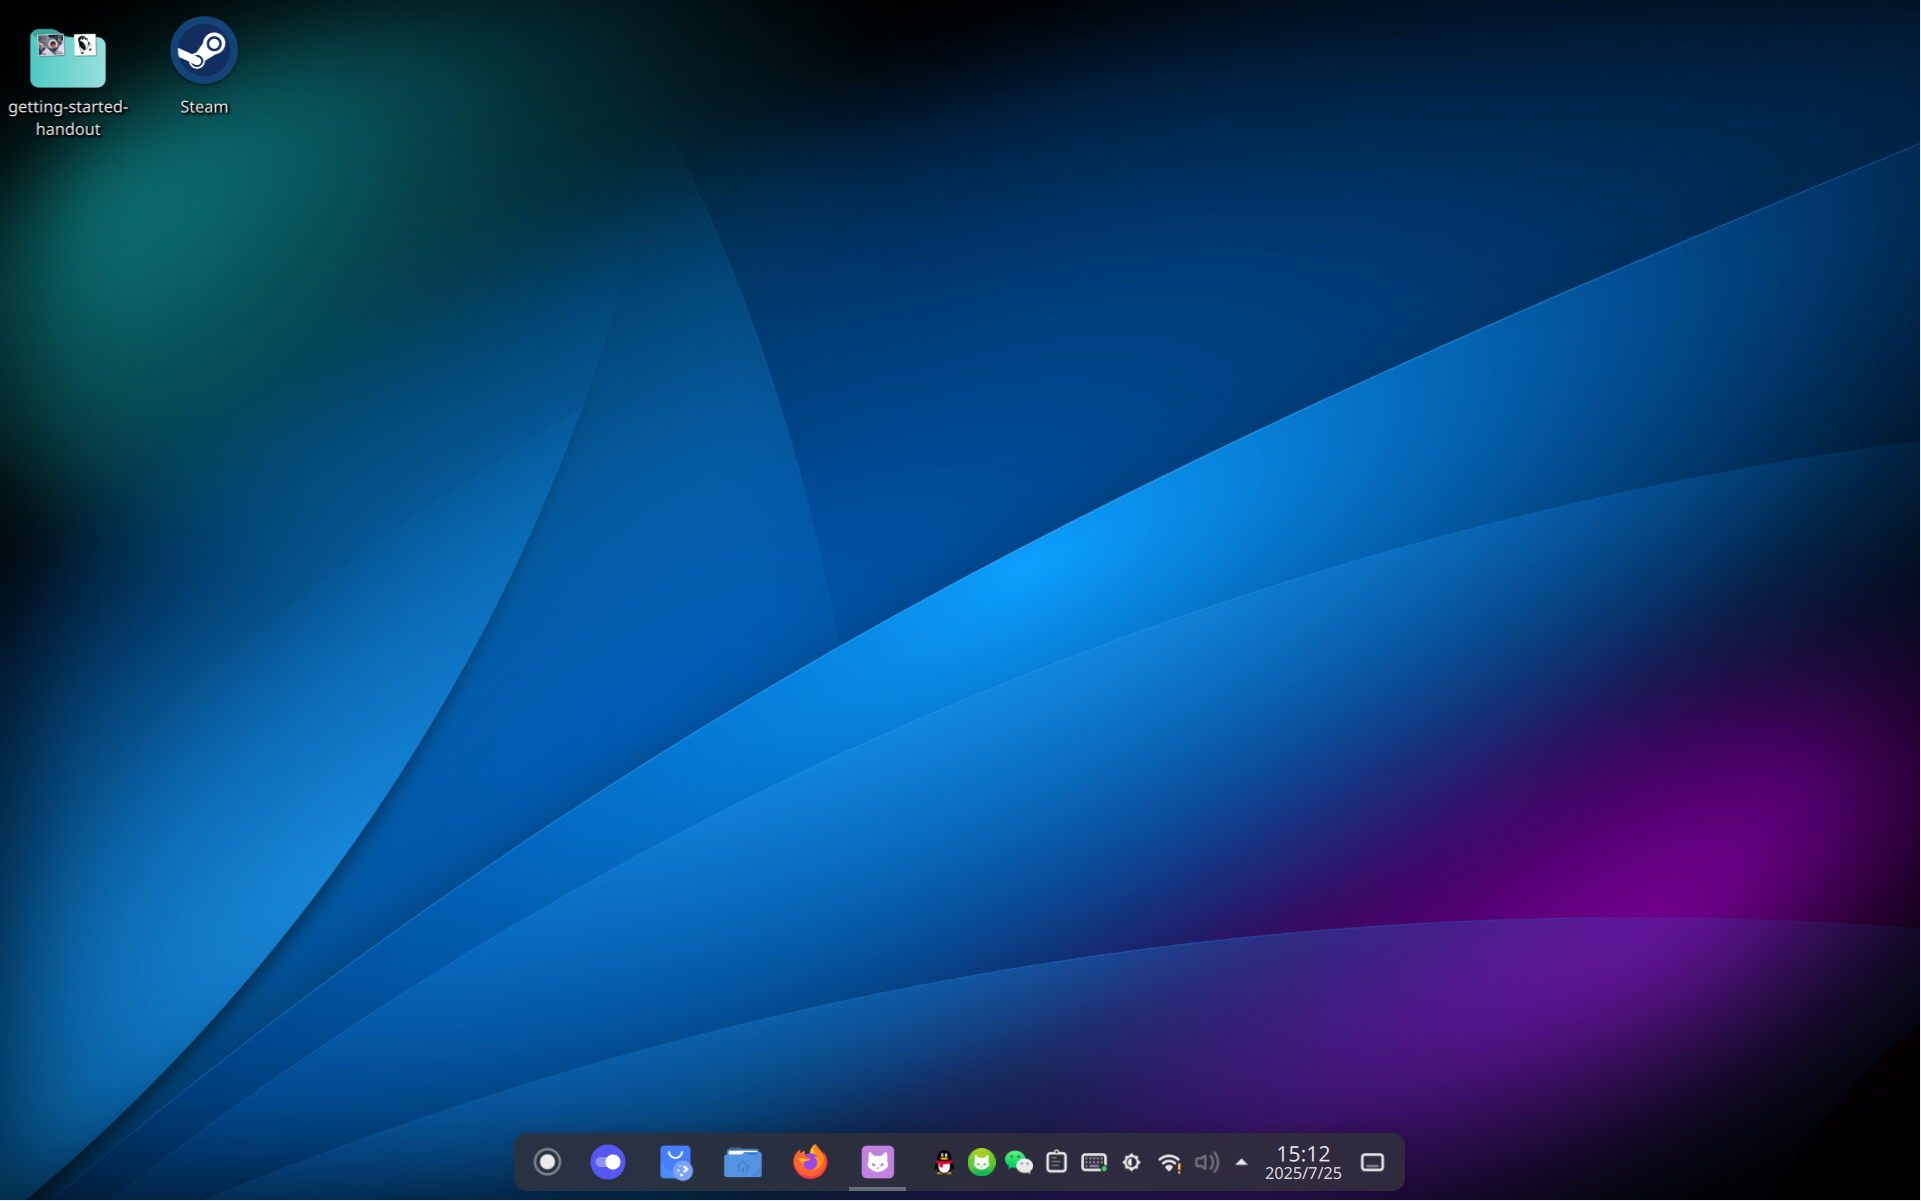
\includegraphics[width=0.8\textwidth]{images/fake-mac.png}
    \caption{一台假装自己是MacOS的ArchLinux机器}
\end{figure}

\subsubsection{驱动程序}

驱动程序是操作系统和硬件之间的桥梁,它负责将操作系统的指令转换为硬件可以理解的语言。驱动程序通常由硬件制造商提供,并且在操作系统安装时自动安装。驱动程序的作用是使操作系统能够正确地识别和使用硬件设备。

驱动程序通常是特定于硬件的,因此不同的硬件设备需要不同的驱动程序。操作系统通常会自动检测硬件设备并安装相应的驱动程序,但是有时候需要手动安装驱动程序。我们可以到软件官网上下载最新的驱动程序,或者使用操作系统自带的驱动程序更新工具来更新驱动程序。不推荐使用“驱动精灵”等第三方驱动程序更新工具,因为它们可能会安装不必要的驱动程序,甚至可能会导致系统不稳定。

\subsubsection{应用软件}

应用软件指的是我们具体用于实现某一功能的工具。这类软件有很多,我们常用的通讯软件QQ、微信等,浏览网页的Chrome、Microsoft Edge等,都是常规软件。
我们下载软件的主要渠道有两种:通过官方渠道下载、通过包管理器(Winget,Homebrew,apt等)下载。这两种渠道一般认为是最安全且问题最少的。

以安装QQ为例,在Windows上,我们需要在腾讯官网上找到QQ的下载页面,然后下载并安装之。在有包管理器的系统(如Linux、macOS)上,我们可以通过包管理器下载,例如\texttt{yay -S linuxqq}(安装了yay的Arch Linux)。我们并不推荐在非官方渠道下载软件,这些非官方渠道往往以某某软件站、某某下载站、某某应用商店(Microsoft Store这类系统自带的除外)等形式出现。通过上述方式下载的软件可能导致使用盗版、附带流氓插件甚至木马、病毒等问题,或者遇到一些其他各种问题。

\subsubsection{北京大学正版软件}

为了保护知识产权、方便学生节约资金,北京大学购买了一系列常用软件的正版授权,方便师生使用。我们可以登录\href{https://software.pku.edu.cn/}{北京大学正版软件网站},使用自己的北大账号和密码登录,下载和安装这些软件。

\subsection{实用软件推荐}

在学习和工作中,我们常常需要一些实用的软件来提高效率。以下是笔者个人推荐的一些实用软件,以供同学们参考。这些软件中有些是免费的,有些是收费的,具体使用时请注意软件的授权和使用条款。同时,为了防止功能冗余,我们非常建议每类软件只安装\textbf{一个}(尤其是播放器和杀毒软件!)。

\begin{itemize}
    \item 下载器类
    \begin{itemize}
        \item Internet Download Manager(IDM):一个极为强大的收费下载软件,可以显著加速下载速度,并支持断点续传等功能。遗憾的是,它不支持磁力链接和BT下载。
        \item Free Download Manager(FDM),一个免费的下载软件,界面友好且现代,且支持磁力链接和 BT 下载。
        \item 比特彗星(BitComet):一个免费且经典的BT下载软件,支持磁力链接和BT下载。
        \item qBittorrent:免费且开源的 BT 下载软件。
    \end{itemize}
    \item 浏览器类
    \begin{itemize}
        \item Google Chrome:一个免费的浏览器,基于Chromium内核。
        \item Mozilla Firefox:一个免费的浏览器,基于Gecko内核。
        \item 油猴:一个浏览器扩展,可以让用户自定义网页的样式和功能。它可以通过安装脚本来实现各种功能,例如广告拦截、界面美化等。油猴支持多种浏览器,包括Chrome、Firefox等。这里推荐一个链接:\href{https://github.com/zhuozhiyongde/PKU-Art}{PKU-Art},它可以给你一个风格现代、足够好看的教学网。
    \end{itemize}
    \item 压缩与解压缩类
    \begin{itemize}
        \item 7-Zip:一个免费且强大的开源老牌压缩软件,支持多种压缩格式,包括7z、zip、rar等。它的压缩率高(7z格式压缩号称全球第一压缩率),速度快,功能强大。
        \item NanaZip:在 7-Zip 基础上提供更现代化的界面(Windows 11 风格),并增加对 ZStd、LZ4 等压缩算法的编解码支持。此外,它使用 MSIX 打包,因此可上架 Microsoft Store,且可以在 Windows 11 的默认右键菜单中直接使用,而无需打开扩展右键菜单。
    \end{itemize}
    \item 播放器类
    \begin{itemize}
        \item VLC Media Player:一个免费的开源播放器,支持众多音频和视频格式。
        \item MPV:免费且开源的播放器,支持格式众多。可以使用命令行、脚本或着色器来精细地控制播放器行为,但上手难度较高。
        \item PotPlayer:另一个免费的播放器。
    \end{itemize}
    \item 杀毒软件类
    \begin{itemize}
        \item Windows Defender:Windows系统自带的杀毒软件,功能强大,查杀率接近100\%,已经和老牌专业杀软(卡巴斯基、BitDefender等)不相上下,能够有效地保护常规情况下计算机免受病毒和恶意软件的侵害。但是误报率较高,可能会误报一些正常的软件为病毒。
        \item 火绒:一个免费的国产杀毒软件,误报率很低,界面友好,适合普通用户使用。然而,火绒的杀毒能力要低一些。
    \end{itemize}
    \item 其他
    \begin{itemize}
        \item Everything:一个免费的文件搜索工具,能够快速地搜索计算机上的文件。它的搜索速度极快,支持多种搜索方式,包括模糊搜索、正则表达式搜索等。
        \item Wallpaper Engine:一个收费的动态壁纸软件,能够让你的桌面变得更加美观。它支持多种动态壁纸,包括视频壁纸、动画壁纸等。
        \item Rufus:一个免费的U盘制作工具,能够将ISO镜像文件写入U盘,制作成可启动的U盘。它支持多种操作系统的ISO镜像,包括Windows、Linux等。
        \item Ventoy:一个开源的u盘启动工具,能够使多个ISO镜像共存于U盘,而不必格式化U盘,选择从其中的一个镜像启动。它能使多个镜像文件和U盘其他文件共存,是装机盘和资料盘合一的好工具。
        \item UltraISO:一个收费的光盘镜像制作工具,能够创建、编辑和转换光盘镜像文件。它支持多种光盘格式,包括ISO、BIN、CUE等。
        \item VMware/VirtualBox:两个免费的虚拟机软件,能够在计算机上创建虚拟机,运行其他操作系统,可以用于测试软件、学习操作系统等。
        \item Cherry Studio:一个LLM管理器,能够帮助你使用各种LLM来简单地创建Agent,来辅助你的开发和生活。
    \end{itemize}
\end{itemize}

\subsection{怎样卸载软件}

我们不推荐反复装卸软件,因为这可能会导致系统不稳定或者软件残留。但是有些时候,我们认为某个软件长期内不会再需要了,且磁盘空间告急,这时我们应该考虑将其卸载。

计算机小白最喜欢做的一件事是把桌面上的快捷方式移动到回收站,这是非常错误的做法。快捷方式只是指向软件的一个链接,删除快捷方式并不会卸载软件本身。对计算机半懂不懂的人喜欢找到软件的安装目录,直接删除软件的文件夹,这也是错误的做法。因为对于许多软件而言,这样做会导致软件的注册表项和其他配置文件残留在系统中,可能会导致系统不稳定或者软件无法正常工作。

正确的做法有两种:要么使用计算机自带的“程序与功能”界面删除软件,要么使用软件自带的卸载程序(通常命名为uninstall.exe或者类似名称)。某些软件可能会在安装时提供一个卸载程序,我们可以在开始菜单或者软件的安装目录中找到它。使用这些方法可以确保软件被完全卸载,留下的残留文件也较少。如要彻底删除残留文件,可以使用一些专业的卸载工具,例如Geek等。

\emph{对于macOS用户而言,卸载软件不需要上文叙述那么麻烦,只需要将应用程序拖到废纸篓中即可!}

\section{计算机间的通讯}

计算机的通讯是指计算机之间或者计算机与其他设备之间进行信息交换的过程。目前计算机间的通讯主要是靠网络来实现的。网络是由许多计算机和其他设备通过通信协议连接在一起的系统,两大要素是\textbf{网络协议}(数据要依赖统一的协议传输)和\textbf{网络设备}(用于连接的设备)。

\subsection{网络基本名词及其解释}

不论是修电脑,还是平常使用计算机联网工作,我们总会在一些场合听到一些网络名词,这些网络名词不乏有被误解的。下面我们将对一些常见的网络名词进行解释。

\subsubsection{IP地址和端口号}
IP地址是计算机在网络中的唯一标识符,类似于“门牌号”。目前有两种通行的IP地址:IPv4和IPv6。IPv4地址是一个32位的二进制数,通常用点分十进制数表示(例如192.168.1.1)。IPv6地址是一个128位的二进制数,通常用冒分十六进制数表示。IPv6地址的引入是为了应对IPv4地址耗尽的问题。

端口号是计算机在网络中用于区分不同应用程序的标识符,类似于“房间号”。端口号是一个16位的整数,范围从0到65535。常见的端口号有80(HTTP)、443(HTTPS)、22(SSH)等。我们假设要指向某一个计算机上的某一个应用程序,那么我们需要指定该计算机的IP地址和端口号。IP地址和端口号一起构成了一个完整的网络地址,通常表示为“IP地址:端口号”(例如0.0.0.0:8000)。

\subsubsection{域名}
域名是计算机在网络中的人类可读的标识符,类似于“网站名称”。域名由多个部分组成,通常用点分隔(例如www.pku.edu.cn)。域名系统(DNS)将域名转换为IP地址,以便计算机可以通过IP地址进行通信。

\subsubsection{子网掩码、网关}

子网掩码是一个32位的二进制数,用于划分IP地址的网络部分和主机部分。它通常用点分十进制数表示,它与IP地址进行按位与运算后,可以得到网络地址。子网掩码的作用是将一个大的网络划分为多个小的子网,以提高网络的效率和安全性。

网关是计算机在网络中的出口,用于连接不同的网络。网关通常是一个路由器或者交换机等设备。

\subsubsection{内网和外网}

我们在日常生活中,常常会听到“内网”和“外网”这两个词。内网是指一个局域网内部的网络,通常用于家庭、学校或者公司等小范围的网络。内网中的计算机可以通过路由器或者交换机等设备连接到外网。外网是指互联网上的网络,通常用于连接不同的局域网和广域网。

内网和外网的IP地址往往是不同的。内网IP地址通常是私有的IP地址,仅在内网中有效(例如每一个地级市都可能有一个“二中”,但是在不同的市称呼“二中”指的不是同一个学校);而外网IP地址全球唯一,互联网可以访问(例如“东港二中”)。例如大名鼎鼎的\texttt{8.8.8.8}是Google的公共DNS服务器的IP地址,它是一个外网IP地址。如果在内网中访问该地址,则可能访问到的不是Google的DNS服务器,而是内网中的某个设备。

\subsubsection{MAC地址}

MAC地址是计算机网络接口的唯一标识符,类似于“身份证号码”。它是一个48位的二进制数,通常用冒分十六进制数表示(例如00:1A:2B:3C:4D:5E)。MAC地址用于在局域网中唯一标识一个设备。每个网络接口卡(NIC)都有一个唯一的MAC地址。MAC地址通常由设备制造商分配,并且在设备的硬件中存储。

\subsubsection{网络协议}

网络协议是计算机之间进行通信的规则和约定。它定义了计算机如何发送和接收数据,以及如何处理错误和异常等情况。常见的网络协议有TCP/IP、HTTP、FTP等。不同的网络协议适用于不同的应用场景,例如TCP/IP协议适用于可靠的数据传输,而HTTP/HTTPS协议适用于Web应用程序的通信、UDP适用于精度要求不太高的实时通信等。

\subsubsection{网络设备}

网络设备是用于连接计算机和其他设备的硬件设备。常见的网络设备有路由器、交换机、集线器等。\textbf{路由器}用于连接不同的网络,并且可以根据网络协议进行数据转发;\textbf{交换机}用于在同一局域网内连接多个设备,并且可以根据MAC地址进行数据转发;\textbf{集线器}用于将多个设备连接到同一个网络,但不具备智能转发功能。

\textbf{光网络单元}(光猫,ONU)是用于将数字信号转换为光信号的设备,通常用于连接到光纤。光猫可以将计算机发送的数据转换为模拟信号,并且将接收到的模拟信号转换为数字信号。我们家用的光纤宽带通常是通过光猫连接到互联网的。

目前家用的路由器往往集成了光猫和交换机的部分功能,因此我们往往不需要像以前一样购买一大堆设备了。

\subsection{校内网络配置指南}

\subsubsection{计算机如何联网}

数据通过网络的传输需要以“数据包”的形式进行。数据包是网络传输的基本单位,它包含了发送方和接收方的IP地址、端口号、数据等信息。数据包通过网络设备(如路由器、交换机等)进行转发,最终到达接收方。

一台具体的机器,进行联网的步骤如下:
\begin{enumerate}
    \item \textbf{物理连接}:使用有线或者无线的方式,将计算机连接到网络设备(如路由器、交换机等)。
    \item \textbf{IP地址分配}:计算机通过DHCP协议自动获取IP地址、子网掩码、网关和DNS等信息。
    \item \textbf{网络协议配置}:计算机根据网络协议栈(如TCP/IP)配置网络协议,确保数据包的正确传输。
    \item \textbf{应用层协议}:计算机通过应用层协议(如HTTP、FTP等)与其他设备进行通信。
    \item \textbf{数据传输}:计算机通过网络设备和协议,将数据包发送到目标设备,并接收返回的数据包。
\end{enumerate}

\subsubsection{有线连接PKU校园网}

我们可以通过有线连接PKU校园网的方式来联网。在宿舍或者有网线接口的地方,我们可以将网线插入计算机的接口,这样就可以直接连接到校园网和互联网。

校园网的网络安全比较一般,建议购买一个路由器,连接到网线接口上,然后通过路由器连接到计算机。这样可以提高网络的安全性和稳定性。

\subsubsection{无线连接PKU校园网}

你可以在支持无线网络的设备WLAN列表中找到以下和北京大学有关的无线网络:
\begin{itemize}
    \item PKU :不安全,不建议使用。
    \item PKU Secure:采用IEEE 802.1x技术,能为用户提供较为安全的加密链路连接,一般情况下建议使用这个网络。
    \item PKU Visitor:访客网络,学生不需要使用这个。
    \item My BJMU:北大医学部的无线网络。
    \item eduroam:全球教育科研网络,该网络可以在全球许多高校使用。
\end{itemize}
具体怎样连接PKU Secure网络,请参考\href{https://its.pku.edu.cn/setting_6.jsp}{PKU Secure连接指南};使用eduroam的同学也可以参考\href{https://its.pku.edu.cn/service_1_eduroam.jsp}{eduroam连接指南}。

\subsubsection{校外连接北大内网}

为方便北京大学校园网用户在校外(家中、出差或国外)访问校园网资源,计算中心提供了VPN服务,可安全地接入校园网,如同在校内一样方便地访问学校全部的内网资源与服务(如校内门户、电子期刊数据资源等)。

具体怎样操作是一件比较复杂的事情,建议参考\href{https://its.pku.edu.cn/service_1_vpn.jsp}{北京大学VPN}的指南进行操作。

\subsubsection{北大网盘}

北大网盘是北京大学为师生提供的云存储服务,用户可以通过北大网盘存储、共享和管理文件。北大网盘提供了大容量的存储空间,并支持多种文件格式的上传和下载。

具体的使用可以参照\href{https://its.pku.edu.cn/service_1_webdisk.jsp}{北大网盘指南}进行操作。

\subsubsection{PKU腾讯会议教育版}

为了解决腾讯会议教育版资源紧张、预约繁琐的问题,计算中心上线了“腾讯会议预约申请”系统。

具体使用可以参照\href{https://its.pku.edu.cn/service_1_webex.jsp}{腾讯会议教育版指南}进行操作。

\emph{腾讯会议教育版只用于学习和工作用途,临时、小规模或其他用途的会议请使用个人账号。}

\subsubsection{北大邮箱及其在第三方客户端的配置(以OutLook为例)}

北京大学为每一个新生都提供了一个北大邮箱。新生的邮箱服务一般由网易提供,地址是\texttt{<学号>@stu.pku.edu.cn}。北大邮箱可以用于接收学校的通知、邮件等信息。

为了方便起见,我们往往习惯于将邮箱配置到第三方客户端(如Outlook、Thunderbird等)上,以便于管理和使用。我将以Outlook为例,介绍如何配置北大邮箱。

首先,打开Outlook,点击“文件”菜单,然后选择“添加账户”。在弹出的窗口中,选择手动进行配置。下文使用IMAP-SMTP协议进行配置。

pku.edu.cn用户:

    接收(IMAP)邮件服务器:\texttt{imap.pku.edu.cn}

    发送(SMTP)邮件服务器:\texttt{smtp.pku.edu.cn}

    在“发送邮件服务器”选项中选定“我的服务器要求身份验证”。

SMTP SSL安全连接使用465端口,IMAP SSL安全连接使用993端口。

stu.pku.edu.cn用户:

    接收(IMAP)邮件服务器:\texttt{imaphz.qiye.163.com}

    发送(SMTP)邮件服务器:\texttt{smtphz.qiye.163.com}

SMTP SSL安全连接使用994端口,IMAP SSL安全连接使用993端口。

在进行正确的配置之后,Outlook会自动连接到北大邮箱服务器,此时会提示你输入用户名和密码。用户名一般是你的邮箱地址。对pku.edu.cn用户而言,密码是你在北大邮箱的登录密码;对stu.pku.edu.cn用户而言,密码应在网易邮箱客户端中获取(登录网易邮箱网页客户端后,\texttt{设置>客户端设置>客户端授权密码})。输入正确的用户名和密码后,Outlook会自动连接到北大邮箱服务器,并开始同步邮件。

\emph{自2025年7月2日始,北京大学邮箱服务建议使用\texttt{pku.edu.cn}域名的用户启用北京大学邮件系统二次验证和客户端专用密码功能。详见\href{https://its.pku.edu.cn/announce/tz20250702100126.jsp}{通知原文},其中也包含了如何启用二次验证和客户端专用密码的说明。}


\section{网安相关知识} % Section Over

\subsection{网络的风险}

虽然互联网的出现给我们带来了便利,但也带来了很多风险。部分人心术不正,使用互联网进行诈骗、盗窃、敲诈勒索等违法犯罪活动;而他们使用的主要手段是不定向的网络攻击,例如钓鱼、木马和病毒等。

钓鱼指的是使用伪造的网页、邮件等方式,诱骗用户输入个人信息,例如用户名、密码、银行卡号等。其目的通常是获取用户的私人信息,以方便对其进行后续的诈骗、勒索等活动。

木马这个词来源于神话中的“特洛伊木马”,原指在一只巨大的木马中藏匿士兵,诱骗敌人打开城门进而发动攻击。现在的木马指一种恶意软件,它伪装成合法的软件或者捆绑在合法软件中,诱骗用户安装。一旦安装,木马就可以在用户不知情的情况下,窃取用户的个人信息、打开端口等。例如,一种最古老且经典的木马是FTP木马,它会在用户的计算机上打开一个FTP端口,允许攻击者远程访问用户的计算机。

蠕虫指的是一种自我复制的恶意软件,它可以在计算机之间传播。蠕虫通常利用计算机系统的漏洞进行传播,一旦感染了一个计算机,就会自动复制自己并传播到其他计算机。蠕虫通常会消耗计算机的资源,导致计算机变得缓慢或者崩溃。一个很经典的蠕虫是“小邮差”,它通过发送带毒邮件进行传播,会占满计算机的网络带宽;一旦感染了计算机,就会自动发送带毒邮件给其他计算机。

病毒指的是一种恶意软件,它可以在计算机之间传播。病毒通常依附在合法的软件中进行传播。病毒通常会破坏计算机的文件、数据等,导致计算机无法正常工作。一个很经典的病毒是“CIH”,它会在每年的4月26日感染计算机,并破坏计算机上的所有文件。它与蠕虫的区别是,病毒不能自己传播,只能依附于其他软件传播;而蠕虫可以自我复制。

被上述恶意软件感染后,计算机会变得不稳定、产生额外的资源开销,甚至导致计算机崩溃、数据破坏,造成经济或其他损失。君子爱财取之有道,我们应该遵纪守法,不要为了炫耀技术或者获取经济利益而制作这些恶意软件。

\subsection{从根源断绝问题}

为了防止计算机受到感染和破坏,最简单的方式是从根源上解决问题。我们在日常使用网络的时候,应该遵循以下原则:

\textbf{不浏览不安全网页}:在浏览网页的时候,若不能确定安全性,则尽量避免浏览不明链接、下载不明文件;如果确实需要下载软件,应该到官方网站上下载。

\textbf{识别伪造网站}:当一个网站需要你输入个人信息时,应该仔细检查该网站的安全性;钓鱼网站通常会伪装成合法网站,例如使用HTTPS协议、与合法网站相似的域名等。我们可以通过查看浏览器地址栏中的锁图标、检查网站的证书、观察域名是否正确等方式来判断网站的安全性。北京大学计算中心每年都会主动制作钓鱼网站,测试本校教职工和学生抗钓鱼的能力。虽然被计算中心骗了是一件不太光彩的事情,也总比被其他人骗了好,至少不会损失钱财。

\textbf{保持系统和软件的更新}:系统和软件的更新有一大部分是安全更新。定期更新软件可以阻止恶意软件利用漏洞进行攻击。

\textbf{保持杀毒软件的自动检测功能开启}:这类检测功能可以帮助我们初步检测计算机上的恶意软件。虽然有时候存在令人诟病的误报,但是它们仍然是我们保护计算机的一道重要防线。

\textbf{使用密钥代替密码}:密钥是一种更安全的身份验证方式,它可以防止密码被窃取。除了常用的公钥-私钥对,密钥还可以是USB设备、手机等。使用密钥可以防止密码被窃取和破解。目前一些技术网站已经支持使用密钥登录,例如GitHub、Google等。而我们在登录远程服务器的时候,也建议使用密钥而非密码登录。

\textbf{使用强密码并定期更换}:如果不得不使用密码登录,建议使用复杂的密码,并定期更换密码。复杂的密码应该包含字母、数字和特殊字符,并且长度至少为8位。我们也可以使用密码管理器(例如BitWarden)来生成和管理复杂的密码。

\textbf{定期备份数据}:定期备份数据可以防止数据丢失和损坏。数据备份有一个321原则:3份数据,2种介质,1个异地备份。也就是说,我们应该至少有3份数据备份,其中2份存储在不同的介质上(例如移动硬盘和云存储),1份存储在异地(例如云存储)。这样,即使我们的数据损坏了,也可以迅速恢复来减少损失。

\textbf{善用沙箱}:沙箱是一种虚拟化技术,可以将应用程序隔离在一个独立的环境中运行。这样可以一定程度上防止恶意软件对计算机造成损害。我们可以使用虚拟机、Docker等工具来创建沙箱环境,对于不能确定安全性的程序可以在此类环境中运行。

\subsection{亡羊补牢,为时未晚}

如果发现自己被钓鱼,应该紧急冻结相关账户并迅速更改密码,防止进一步的经济损失。在接下来的一个月到数个月中务必慎之又慎,你的信息可能已经被泄露,招致电信诈骗的概率显著增高。

如果发现自己的计算机感染了木马、病毒、蠕虫等,此事比被钓鱼更加严重。你应该依次执行以下内容:

\begin{itemize}
    \item \textbf{立即结束进程}:如果你能定位具体是哪一个软件正在搞破坏,可以使用任务管理器结束该进程。不过大多数情况下我们无法确定具体是哪一个进程出问题,此时忽略这一步即可。
    \item \textbf{立即断网}:这是一种负责任的行为,可以防止病毒进一步扩散。仅在软件层面上切断网络并不足够,如果你的计算机使用有线网络应该拔掉网线,以防止恶意进程重新连接网络。
    \item \textbf{立即查杀}:你可以运行杀毒软件的查杀功能,如是旧种类的病毒,杀毒软件应对起来不会太难。
    \item \textbf{立即上报}:如果杀毒软件查杀失败,应该立即上报相关部门。这可能意味着新型病毒的出现,上报有关部门有利于他们做出迅速反应,可以减少损失。
    \item \textbf{立即重装系统}:彻底重新格式化硬盘并重装系统可以彻底地清除残留的病毒文件。这是没有办法的办法,但却是最有效的。
\end{itemize}

\end{document}